\bigskip
\begin{center}\textsc{Gauss} an \textsc{Gerling}.\quad Göttingen, 5. Juni 1838.\end{center}

Nach einem Satz, von dem ich nicht sicher weiß, ob ich ihn Ihnen früher
schon mitgeteilt habe, muss man, wenn in einem Dreieckssystem $p$ Punkte
durch $l$ Linien verbunden sind, unabhängig davon, ob deren Richtungen
nur einseitig oder in beiden Richtungen festgelegt sind, außer den Bedin-\par
\makeatletter
\def\ps@gaussIXfortyonestar{\def\@oddhead{}\def\@evenhead{}\def\@oddfoot{\hfil41\textsuperscript{*}\hspace{2em}}\let\@evenfoot\@oddfoot}
\makeatother
\thispagestyle{gaussIXfortyonestar}
\clearpage
\noindent324\hfill\textbf{BRIEFWECHSEL.}\par\medskip
\noindent gungsgleichungen der (ersten und) zweiten Klasse [den Horizontabschlüssen
und den Winkelgleichungen] noch $l-2p+3$ voneinander unabhängige Bedingungsgleichungen
erhalten. \textls[120]{Weder mehr noch weniger.} Es kann allerdings vorkommen, dass
sich diese nicht alle in die Form der dritten Klasse [der Seitengleichungen]
bringen lassen, etwa bei einem Ring von Dreiecken.
\begin{center}
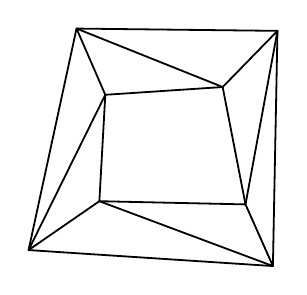
\begin{tikzpicture}[x=.58cm,y=.58cm,line width=.65pt,line cap=round,line join=round]
\coordinate (A) at (1.05,5.3);
\coordinate (B) at (5.45,5.25);
\coordinate (C) at (5.35,0.1);
\coordinate (D) at (0,0.45);
\coordinate (E) at (1.68,3.85);
\coordinate (F) at (4.25,4.02);
\coordinate (G) at (4.75,1.45);
\coordinate (H) at (1.55,1.52);
\draw (A)--(B)--(C)--(D)--cycle;
\draw (E)--(F)--(G)--(H)--cycle;
\draw (A)--(E) (A)--(F) (B)--(F) (B)--(G)
      (C)--(G) (C)--(H) (D)--(H) (D)--(E);
\end{tikzpicture}
\end{center}

Ich lasse diese Ausnahme jedoch außer Betracht, da sie bei Ihrem System
nicht berücksichtigt werden muss.

Ich zähle nun
\[
\begin{aligned}
p&=24\ \text{Punkte}\\
l&=66,\ \text{nämlich }\begin{aligned}[t]22\ &\text{einseitige Richtungen,}\\44\ &\text{konjugierte Richtungen,}\end{aligned}
\end{aligned}
\]
sodass es 21 der fraglichen Bedingungsgleichungen geben muss, und so viele
haben Sie tatsächlich. Die Unabhängigkeit lässt sich prüfen, indem man die
$p$ geeignet anordnet, wobei ich von der Reihenfolge Ihrer Zahlen
1 .\ .\ .\ .\ 112 teilweise abweichen musste, und denselben Satz wiederholt
anwendet, während man nach und nach alle $p$ Punkte hinzunimmt. Auch diese
Prüfung haben Ihre 21 Gleichungen bestanden. In \textls[120]{Ihrer}
Nummerierung gibt es einige Unstimmigkeiten. 24 und 61 fehlen, sodass sich
insgesamt (wie oben $22+2\mathbin{.}44)=110$ Richtungen ergeben, und 112
steht an der falschen Stelle.

Nach dieser Prüfung zweifle ich nicht daran, dass Sie Ihre 21 Gleichungen
unbesorgt vorlegen können.

Wenn ich richtig gezählt habe, müssen Sie außerdem 24 Bedingungsgleichungen
der $2^{\mathrm{ten}}$ Klasse haben.

Auf einen Punkt bei der Ausführung muss ich Sie noch aufmerksam machen.
Falls ich das schon früher getan habe, möge die gute Absicht meine
Vergesslichkeit entschuldigen.

Bei der Aufstellung Ihrer Tabellen weichen Sie insofern von meiner Form ab,
als Sie alle Richtungen von \textls[120]{einer von ihnen} aus zählen, während ich
von einer gewissermaßen willkürlichen, genauer gesagt einer dem System\par
\clearpage
\noindent\textbf{ZUR NETZAUSGLEICHUNG.}\hfill325\par\medskip
\noindent fremden Richtung aus zähle. Sie dürfen daher bei der Ausführung
nicht vergessen, dass sämtliche Richtungen gleich zuverlässig oder,
genauer gesagt, gleich unzuverlässig sind und dass Sie also Ihre jeweilige
0 zu den zu korrigierenden Richtungen zählen müssen. Das Ergebnis wird
stets sein, dass die Summe aller Korrekturen an einem Standpunkt $=0$ wird.

\begingroup
\def\letterfivestars{*}
\makeatletter
\renewcommand{\@makefnmark}{\hbox{\normalfont[\textsuperscript{\letterfivestars})]}}
\renewcommand{\@makefntext}[1]{\parindent1em\noindent\hbox to2.4em{\hss[\textsuperscript{\letterfivestars})\ }#1]}
\makeatother
Ich bewundere aber Ihre Unerschrockenheit, eine so große Eliminationsarbeit
zu übernehmen. Den gleichen Mut hätte ich nicht gehabt. Bei meinen 33
Punkten war die Anzahl der Bedingungsgleichungen der $3^{\mathrm{ter}}$ Klasse
[der Seitengleichungen] viel kleiner (ich glaube 7)\footnote{Es sind 12.}.
Beschränkte man sich anfangs auf die Gleichungen der $2^{\mathrm{ten}}$ Klasse
[der Winkelgleichungen], war die Elimination trotz der großen Zahl dieser
Gleichungen auf indirektem Weg leicht, und Rechenfehler waren unmöglich. Da
sämtliche Richtungen hin und zurück gemessen worden waren, ließen sich
Änderungen vornehmen, die die Arbeit sehr erleichterten und rasch zu
stabilen Ergebnissen führten. Ich fürchte, dass Letzteres bei Ihnen in
viel geringerem Maß der Fall sein wird\def\letterfivestars{**}\footnote{Vgl. S.\ 250/251.}.
Wenn Sie sich aber das Ziel einmal gesetzt haben, bleiben Ihnen als Mittel
nur Aufmerksamkeit und Geduld.

Hätte ich diese Rechnungen selbst durchführen müssen, so hätte ich die drei
Orte, an denen nicht gemessen wurde, gar nicht in das System aufgenommen,
nicht weil ich das missbillige, sondern weil ich die große Arbeit gescheut
hätte. Wenn alle nur einseitig beobachteten Richtungen ausgeschlossen
würden, wäre die Ausgleichung des Systems sehr leicht. Allerdings gewinnt
bei Ihrem Vorhaben die Sicherheit durch die vollständige Berücksichtigung
erheblich. .\ .\ .\ .\ .\ .

Die Anordnung bei den Vierecken ist im Übrigen an sich willkürlich. Nur um
diese Willkür auszuschließen, befolge ich die von Ihnen zitierte
Regel\def\letterfivestars{***}\footnote{Vgl. den Brief an \textsc{Gerling} vom 11. Februar 1824, S.\ 249. \textsc{Gerling} hatte dazu
(am 2. Juni 1838) geschrieben: »Ich habe mir über den Grund der Regel bisher nur
insofern Rechenschaft geben können, als auf diese Weise verhältnismäßig die größten
Koeffizienten zum Vorschein kommen.«}, die außer dem von Ihnen richtig
erratenen keinen weiteren Vorzug hat.
\endgroup
